\documentclass[t]{sdqbeamer}
%\documentclass[c]{sdqbeamer}

\usepackage{listings}
\usepackage{graphicx}
\usepackage{tabularx}
\usepackage{tikzsymbols}

\hypersetup{
	colorlinks=true,
	urlcolor=kit-orange
}

% set sdqbeamer options
\titleimage{blender-render}
\groupname{Algorithm Engineering}
\grouplogo{ae}
\selectlanguage{english}

% define title etc.pp.
\title[SAT Solving]{Practical SAT Solving}
\subtitle{Lecture 2}
\author{\underline{Markus Iser}, Dominik Schreiber, Tom\'a\v{s} Balyo}
\date{April 22, 2024}

% Existing KIT colors: kit-green, kit-blue, kit-red, kit-gray, kit-orange, kit-lightgreen, kit-brown, kit-purple, kit-cyan
% configure appearance
\setbeamercolor{block title}{bg=kit-blue}
\setbeamercolor{block body}{bg=kit-blue!10}
\setbeamercolor{block title example}{bg=kit-orange}
\setbeamercolor{block body example}{bg=kit-orange!10}
\setbeamertemplate{itemize item}{\color{kit-gray}\textbullet}
\setbeamertemplate{itemize subitem}{\color{kit-gray}\textbullet}
\setbeamercolor{item projected}{bg=kit-gray, fg=kit-gray}
\renewcommand{\insertnavigation}[1]{} % remove navigation bar

% define commands
\definecolor{myblue}{HTML}{0D3B66}
\definecolor{myred}{HTML}{6E0E0A}
\definecolor{mypink}{HTML}{F7B2B7}

\newcommand{\vars}[1]{\textsf{vars} (#1)}
\newcommand{\lits}[1]{\textsf{lits} (#1)}
\newcommand{\clss}[1]{\textsf{clss} (#1)}

\newcommand{\highl}[1]{\textcolor{myblue}{#1}}
\newcommand{\highlo}[1]{\textcolor{myred}{#1}}
\newcommand{\highlow}[1]{\textcolor{mypink}{#1}}

% Extra column types for tabularx
\newcolumntype{C}{>{\centering\arraybackslash}X}
\newcolumntype{L}{>{\raggedright\arraybackslash}X}
\newcolumntype{R}{>{\raggedleft\arraybackslash}X}

\newcommand{\setcolsep}[1]{\setlength{\tabcolsep}{#1}}
\newcommand{\setrowsep}[1]{\renewcommand{\arraystretch}{#1}}

% Definitions for the Tseitin transformation
\newcommand{\true}{\ensuremath{\mathit{True}}}
\newcommand{\false}{\ensuremath{\mathit{False}}}
\newcommand{\allvars}{\ensuremath{\mathcal{V}}}
\newcommand{\tseitin}[1]{\ensuremath{\mathcal{T}(#1)}}
\newcommand{\tseitinRec}[2]{\ensuremath{\mathcal{T}^{#2}(#1)}}
\newcommand{\tseitinSym}[1]{\ensuremath{\mathcal{T}_\mathsf{lit}(#1)}}
\newcommand{\tseitinDef}[2]{\ensuremath{\mathcal{T}_\mathsf{def}^{#2}(#1)}}
\newcommand{\hcancel}[2][black]{\setbox0=\hbox{$#2$}\rlap{\raisebox{.45\ht0}{\textcolor{#1}{\rule{\wd0}{1pt}}}}#2} 
\newcommand{\sateq}{\mathrel{\overset{\makebox[0pt]{\mbox{\normalfont\tiny\sffamily SAT}}}{=}}}

\newcommand{\enc}{\ensuremath{\mathcal{E}}} % encoding

% exercise commands
\newcommand{\exhead}[3]{
\hrule~\\[1ex]\noindent
{\bf Practical SAT Solving} (ST 2024) \hfill \fbox{Assignment #1} \\[1ex]
Markus Iser, Dominik Schreiber, Tom\'a\v{s} Balyo\\[1ex]
Algorithm Engineering (KIT) \hfill #2 -- #3\\
\hrule
\thispagestyle{empty}
}
\setlength{\itemsep}{1em}

\begin{document}

\begin{frame}
	\thispagestyle{empty}
	\titlepage
\end{frame}

\begin{frame}{Overview}
	\begin{block}{Recap. Lecture 1}
		\begin{itemize}\setlength{\itemsep}{1em}
			\item Satisfiability: Propositional Logic, CNF Formulas, NP-completeness, Applications
			\item Examples: Pythagorean Triples, Arithmetic Progressions, k-Colorability
			\item Incremental SAT: IPASIR, Sample Code
		\end{itemize}
	\end{block}
	\begin{block}{Today's Topics}
		\begin{itemize}\setlength{\itemsep}{1em}
			\item Tractable Subclasses
			\item Constraint Encodings
			\item Encoding Techniques
		\end{itemize}
	\end{block}
\end{frame}

\begin{frame}{Tractable Subclasses}
\begin{block}{Tractable Subclasses \href{https://doi.org/10.1145/800133.804350}{(cf.~Schaefer, 1978)}}
	\begin{itemize}\setlength{\itemsep}{1em}
		\item \textbf{2-SAT}\\Exactly two literals per clause
		\item \textbf{HORN-SAT}\\At most one positive literal per clause
		\item \textbf{Inverted HORN-SAT}\\At most one negative literal per clause
		\item \textbf{Positive / Negative}\\Literals occur only pure (either positive or negative)
		\item \textbf{XOR-SAT}\\No clauses, only XOR constraints
	\end{itemize}
\end{block}
\end{frame}

\begin{frame}{2-SAT}
Each clause has exactly two literals.
\begin{example}[2-SAT Formulas]
\vspace*{-3ex}
\begin{flalign*}
	F_5 &= \{ \{ x_1, x_2 \}, \{ \overline{x_1}, x_2 \}, \{ x_1, \overline{x_2} \}, \{ \overline{x_1}, \overline{x_2} \} \} &\\
	F_7 &= \{ \{ \overline{x_1}, x_2 \}, \{ \overline{x_2}, x_3 \}, \{ \overline{x_3}, x_1 \}, \{ x_2, x_4 \}, \{ x_3, x_4 \}, \{ x_1, x_3 \} \} &
\end{flalign*}
\end{example}
\begin{block}{Linear Time Algorithm for 2-SAT \href{https://doi.org/10.1016/0020-0190(79)90002-4}{(cf.~Aspvall et al., 1979)}}
	\begin{itemize}\setlength{\itemsep}{1em}
		\item Construct Implication Graph
		\item Find Strongly Connected Components (SCC) with Tarjan's Algorithm\\
			  Complexity: $\mathcal{O}(n+m)$, where $m$ is the number of clauses
		\item Check for Complementary Literals in the same SCC
	\end{itemize}
\end{block}
\end{frame}

% \begin{frame}{How to solve 2-SAT?}
% \begin{block}{Saturation Algorithm}
% The resolution saturation algorithm is \highl{polynomial} for 2-SAT.
% \end{block}
% \textbf{Proof}
% \begin{itemize}
% 	\item Only 2-literal resolvents are possible
% 	\item There are only $\mathcal{O}(n^2)$ 2-literal clauses on $n$ variables
% \end{itemize}
% \textbf{Complexity}
% \begin{itemize}
% 	\item Both time and space $\mathcal{O}(n^2)$
% 	\item There exists a \highl{linear algorithm}! \cite{aspvall1979linear} \\($\mathcal{O}(n+m)$, where
% 	$m$ is the number of clauses)
% \end{itemize}
% \end{frame}

\begin{frame}{Implication Graph}
	An \textbf{implication graph} of a 2-SAT formula $F$ is a \highl{directed graph} with a vertex for each literal of $F$ and 2 edges for each clause $(l_1 \vee l_2)$: $\overline l_1 \rightarrow l_2$ and $\overline l_2 \rightarrow l_1$.
\begin{example}[Implication Graph]
	\centering
	\vspace*{1ex}
	\begin{columns}[T]
	\begin{column}{0.6\textwidth}
		$F_7 = \{ \{ \overline{x_1}, x_2 \}, \{ \overline{x_2}, x_3 \}, \{ \overline{x_3}, x_1 \}, \{ x_2, x_4 \}, \{ x_3, x_4 \}, \{ x_1, x_3 \} \}$\\[1ex]
		\only<2>{
			\begin{itemize}\setlength{\itemsep}{1em}
				\item Find \highl{Strongly Connected Components} (SCC)
				\item SCC: There is a path from every vertex to every other vertex
				\item \highl{Tarjan's algorithm} finds SCCs in $\mathcal{O}(|V|+|E|)$
			\end{itemize}
		}
		\only<3->{
			\begin{itemize}\setlength{\itemsep}{1em}
				\item If an SCC contains both $x$ and $\overline{x}$, the formula is \highlo{UNSAT}
				\begin{itemize}\setlength{\itemsep}{1ex}
					\item $x$ implies its own negation!
					\item Literals in an SCC must be either all true or all false
				\end{itemize}
				\item<4> What about \highlo{SAT}? How to get a solution?
				\begin{itemize}\setlength{\itemsep}{1ex}
					\item Contract each SCC into one vertex
					\item In reverse topological order, set unassigned literals to \texttt{true}.
					% \item Example: $x_1 = x_2 = x_3 = \texttt{true}$, $x_4 = \texttt{true}$, the rest is already assigned.
				\end{itemize}
			\end{itemize}
		}
	\end{column}%
	\begin{column}{0.3\textwidth}
		\only<1>{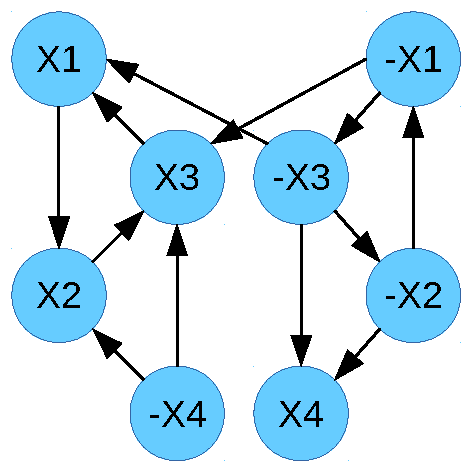
\includegraphics[width=.9\textwidth]{figures/l02/impgraph.pdf}}
		\only<2-3>{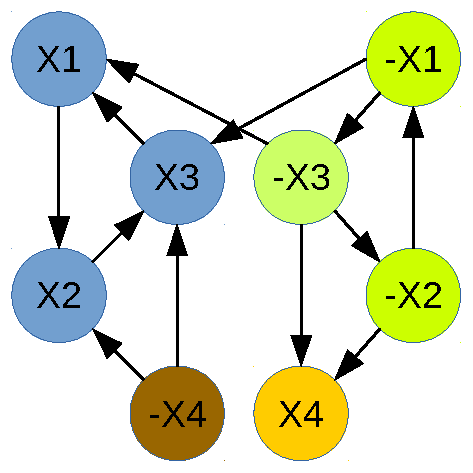
\includegraphics[width=.9\textwidth]{figures/l02/impgraph-comp.pdf}}
		\only<4>{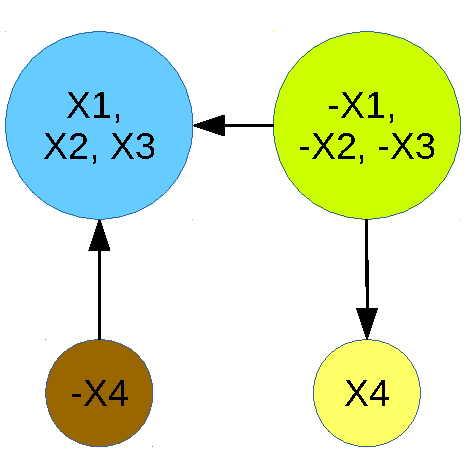
\includegraphics[width=.9\textwidth]{figures/l02/impgraph-cond.pdf}}
	\end{column}
	\end{columns}
\end{example}
\end{frame}


\begin{frame}{HornSAT}
	Each clause contains at most one positive literal.
	\begin{example}[Horn Formula]
		Each clause can be written as an implication with \highl{positive literals only and a single consequent}:
		\vspace*{-1ex}
		\begin{flalign*}
			F_6 &= \bigl\{ \{ \overline{x_1}, x_2 \}, \{ \overline{x_1}, \overline {x_2}, x_3 \}, \{ x_1 \} \bigr\} &\\
				&\equiv \bigl(x_1 \rightarrow x_2\bigr) \wedge \bigl((x_1 \wedge x_2) \rightarrow x_3\bigr) \wedge \bigl(\top \rightarrow x_1\bigr) &
		\end{flalign*}
	\end{example}
	\pause
	\begin{block}{Solving Horn Formulas}
		\begin{itemize}
			\item Propagate until fixpoint
			\item If $\top \rightarrow \bot$ then the formula is \highlo{UNSAT}. Otherwise it is \highl{SAT}.
			\item Construct a satisfying assignment by setting the remaining variables to \texttt{false}
		\end{itemize}
	\end{block}
\end{frame}

\begin{frame}{Hidden / Renamable / Disguised Horn}
	A CNF formula is \highl{Hidden Horn} if it can be made \highl{Horn} by flipping the polarity of some of its variables.
	\begin{example}[Hidden Horn Formula]
		\vspace*{-3ex}
		\begin{flalign*}
			F_8 = &\{ \{ x_1, x_2, x_4 \}, \{ x_2, \overline{x_4} \}, \{ x_1 \} \} &\\
			\leadsto &\{ \{ \overline{x_1}, \overline{x_2}, x_4 \}, \{ \overline{x_2}, \overline{x_4} \}, \{ \overline{x_1} \} \} &
		\end{flalign*}
	\end{example}
	\highl{How to recognize} a Hidden Horn formula? \highlo{And how to hard is it?}
	\pause
	\begin{block}{Recognizing Hidden Horn Formula $F$}
		Construct 2-SAT formula $R_F$ that contains the clause $\{l_1, l_2\}$ iff there is a clause $C \in F$ such that $\{l_1, l_2\} \subseteq C$.\\[1ex]
		\begin{itemize}\setlength{\itemsep}{1em}
			\item Example: $R_{F_8} = \{ \{ x_1, x_2 \}, \{ x_1, x_4 \}, \{ x_2, x_4 \}, \{ x_2, \overline{x_4} \} \}$
			\item If the 2-SAT formula is satisfiable, then $F$ is Hidden Horn
			\item If $x_i = \texttt{true}$ in $\phi$, then $x_i$ needs to be renamed to $\overline x_i$
		\end{itemize}
	\end{block}
\end{frame}

\begin{frame}{Mixed Horn}
	A CNF formula is \highl{Mixed Horn} if it contains only binary and Horn clauses.
	\begin{example}[Mixed Horn Formula]
		\vspace*{-3ex}
		\begin{flalign*}
			F_9 = &\{ \{ \overline{x_1}, \overline{x_7}, x_3 \}, \{ \overline{x_2}, \overline{x_4} \}, \{ x_1, x_5 \}, \{ x_3 \} \} &
		\end{flalign*}
	\end{example}
	\highl{How to solve} a Mixed Horn formula? \highlo{And how to hard is it?}
	\pause
	\begin{block}{Mixed Horn is NP-complete}
		\textbf{Proof}: \highl{Reduce SAT} to Mixed Horn SAT
		\begin{itemize}\setlength{\itemsep}{1em}
			\item For each non-Horn non-quadratic clause $C=(l_1 \vee l_2 \vee l_3 \vee \dots)$
			\begin{itemize}\setlength{\itemsep}{1ex}
				\item for each but one positive $l_i$ $\in C$ introduce a new variable $l'_i$
				\item replace $l_i$ in $C$ by $\overline{l'_i}$
				\item add $(l'_i \vee l_i) \wedge (\overline{l'_i} \vee \overline{l_i})$ to establish $l_i = \overline{l'_i}$
			\end{itemize}
		\end{itemize}
	\end{block}
\end{frame}

\end{document}
